\documentclass[tikz]{standalone}
\usepackage{tikz}
\usetikzlibrary{matrix,fit,backgrounds,calc,decorations.markings,arrows.meta,shapes.geometric}
\usepackage{amsmath}
\usepackage{braket}

\begin{document}
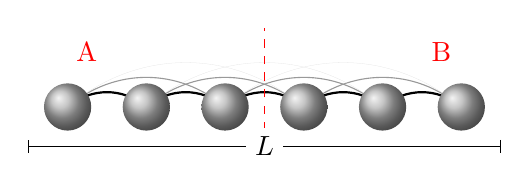
\begin{tikzpicture}
	% \draw[->] (0, 0) -- (5., 0) ;
	\foreach \i in {0,...,4}
		\draw[thick,color=black] (\i,0) to[in=140,out=40] +(1,0);
	\foreach \i in {0,...,3}
		\draw[color=black!40] (\i,0) to[in=140,out=40] +(2,0);
	\foreach \i in {0,...,2}
		\draw[ultra thin,color=black!10] (\i,0) to[in=140,out=40] +(3,0);
	\foreach \i in {0,...,5} {
		\shade[ball color=black!30!white] (\i, 0) circle [radius=0.3] ;
		% \draw[fill=black!30!white] (\i, 0) circle [radius=0.3] ;
	}
	\draw[thin,dashed,red]    (2.5,-0.3) -- (2.5,1.0);
	\node[red,left]  at (0.5, 0.7) {A};
	\node[red,right] at (4.5,0.7) {B};
	\draw[|-|] (-0.5,-0.5) -- (5.5,-0.5) ;
	\node[fill=white] at (2.5,-0.5) {$L$};
\end{tikzpicture}
\end{document}
